\section{Component Interfaces}

\subsection{Backend APIs}
In this section the main APIs that the back-end application will expose are shown and commented. They are grouped according to the entities they are mostly related to.

\subsubsection{User APIs}
These APIs will handle the data related to the User entity, therefore their route will be prefixed by “/user”. They'll retrieve all necessary data to display the profile of a user, including the points obtained in SafeStreets reward system. Some of these APIs will be accessible only to the user they are related to, others will also be available to authorities.

\subsubsection{Login APIs}
These APIs will manage the access to the system for both standard users and authorities. Their route will be prefixed by “/login”. Login APIs are accessible to anyone who is not already logged in, as it is their role to check the validity of user credentials and, in case they are correct, generate tokens that allow the logged user to access other areas of the application.

\subsubsection{Registration APIs}
These APIs will allow visitors to register to SafeStreets and authorities to upgrade their profile. Their route will be prefixed by “/register”. Registration APIs are accessible to all visitors that are not logged in the application.

\subsubsection{Report APIs}
These APIs will manage the creation and validation of reports. All APIs belonging to this group will be prefixed by “/report”. Report APIs are only available to users that have a verified profile; some of these APIs will only become available to specific profiles (e.g. the APIs that allow to vote for the approval of a report).

\subsubsection{Ticket APIs}
These APIs will handle the generation of tickets and therefore all their routes will be prefixed by “/ticket”. These APIs are only available to verified authorities.

\subsubsection{Statistics APIs}
These APIs will retrieve all necessary data to display the maps of safe and unsafe areas. Their routes will be prefixed by “/stats”. The majority of these APIs are accessible to anyone, but a few are available only to authorities as they retrieve specific data about offenders.
\newline
\newline
In the following page an overview of the main APIs and respective server-side controllers is provided.
\newpage
\begin{figure}[H]
  \centering
  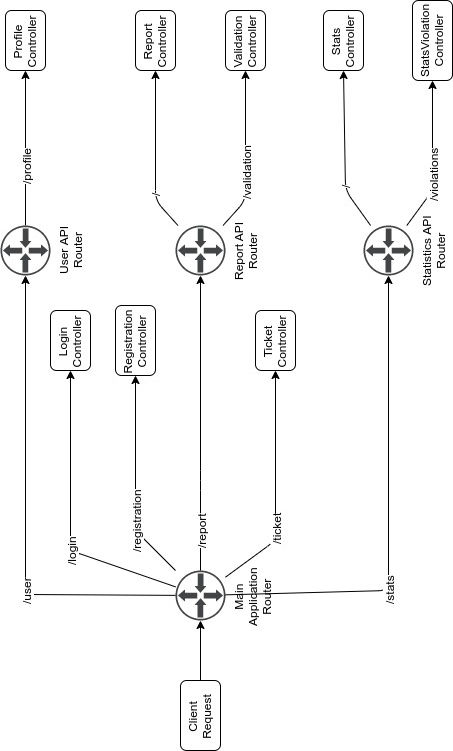
\includegraphics[origin=c,width=\textwidth,height=.95\textheight,keepaspectratio]{DD_Images/ComponentInterface/InterfaceDiagram.jpg}
  \caption{\textit{Interface Diagram}}
\end{figure}